%----------------------------------------------------------------------------
\chapter{Implementáció}
%----------------------------------------------------------------------------

\section{Tanítóadatok előkészítése}

A letöltött tanítóadatokat NeMo által értelemzhető formátumúra kellett hozni. Ez magába foglalta a fájlok konvártálását .wav formátumba. Az egyes tanítóadatok más-más formátumban (.opus, .flac, .mp3) voltak eredetileg, illetve eltérő fájstruktúrákba voltak szervezve.

A konvertáláshoz a fentiek miatt a python os könyvtárának walk metódusát használtam mellyel egy mappát rekúrzívan be lehet járni. A konvertáláshoz az ffmpeg szoftvert használtam, mivel segítségével több formátum is könnyedén konvertálható .wav formátumba.

A fájlok átalakításán kívül szükséges volt az adatok .json fájljainak elkészítése, mely megmondja, hogy melyik hangfájl hol található, milyen hosszú és mi hangzik el rajta. A NeMo-nak ezután csupán az egyes manifest-eket, .json fájlokat, kellett megadni, azzal a kiegészítéssel, hogy melyiket kívánjuk tanító vagy teszt adathalamznak használni, és a további előfeldolgozási lépéseket már autómatikusan elvégezte. Természetesen több információ tárolását is támogatja a NeMo, de ezek az adatok elengedhetetlenek.

\section{Modellek kimentése és betöltése}

A tanított modelleket el kell menteni későbbi használat végett. Két módszert is alkalmaztam. Az egyik a logoláshoz hasonlóan callback-et használ, mindig a legoptimálisabb eredményt elért epochot menti ki .ckpt fomrátumban, míg az utóbbi módszer a tanítás végén menti ki a modellt .nemo formátumban.

A mentésre a későbbi felhasználás meleltt azért is van szükség, mert a hosszú tanításokat, melyek akár 48 órán át is tarthatnak, szükséges lehet megszakítani. A megszakítás után fontos úgy betölteni a modellt, hogy az továbbtanítható legyen. A NeMo külön kezeli a modellt és a tanítást végző trainert, melykbe külön külön szükséges betölteni a folytatni kívánt checkpoint-ot.

\section{Kalibráció angol nyelv segítségével}

Első lépésként egy kisebb adatbázison, az AN4-en teszteltem a NeMo keretrendszert, a Google Colab segítségével. Az alap paraméterekkel és konfigurációval az elért eredmények elmaradtak a referencia eredményekéhez képest. Az AN4-es tanítás során QuartzNet 5x1-es architektúrájával dolgoztam a kevés mennyiségű adat végett.

A pontosság növelése érdekében az egy gyakran használt módszer az epoch szám növelése. Egy epoch reprezentálja az összes tanítóadaton való kiértékelést és a súlyok javítását a hiba tükrében. Magas epoch szám jobb eredményeket produkál, de vigyázni kell, mert túlzott epoch szám esetében megjelenhet az úgy nevezett túltanítás jelenség. Ez annyit tesz, hogy a túlzottan is megtanulja a modell a tanítóadatokat, azokra nagyon jó eredményt ad, míg általánosan egyre rosszabbul teljesít.

Egy másik fontos paraméter aminek a módosításával növelni lehet az elért pontosságot a learning rate. A learning rate felel a hiba nyomán felmerült tanítás, azaz súlyok korrekciójának mértékéért. Túl nagy lépések, javítások, esetén a loss értéke, amit csökkenteni szeretnénk, túl nagy ugrásokat végez, akár a rossz irányba. Túl alacsony érték esetén lassan éri el a loss a minimum pontját, legyen az globális vagy lokális, ahogy az az 51-es ábrán látható. Szintén nem kívánt eredmény az alacsony learning rate esetén, hogy a loss értéke ideje korán beragad egy lokális minumum értékben, ami egy nagyobb lépéssel áthidalható lenne.

\begin{figure}[!ht]
\centering
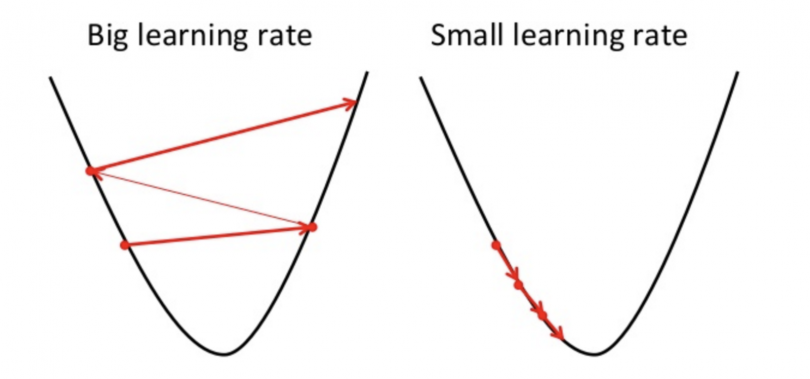
\includegraphics[width=150mm, keepaspectratio]{figures/gradient-descent-learning-rate.png}
\caption{Learning Rate fontossága, \url{https://builtin.com/data-science/gradient-descent}.}
\end{figure}

A fentiek tükrében növeltem az epoch számot és a learning rate-et, 200-ra és 0.02-re. Sikerült egy optimálisabb eredményt elérjek, így a felhasznált paraméterekkel tovább tudtam indulni egy nagyobb adatbázison való tesztelésre.

\begin{figure}[!ht]
\centering
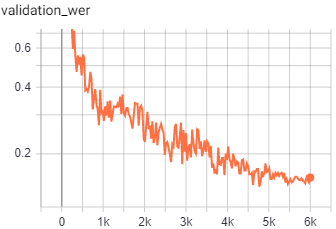
\includegraphics[width=100mm, keepaspectratio]{figures/an4_wer.png}
\caption{AN4 adatbázis validációs adathalmazán elért eredmények.}
\label{fig:TeXstudio}
\end{figure}

Arról, hogy a beállításaim tényleg megfelelőek a LibriSpeech 100 órás adathalmazán bizonyosodtam meg. Azért nem ezzel kezdtem, mert 100 órányi hanganyag tanítása jóval tovább tart, így minél kevesebbszer akartam végigfuttatni a tanítást az optimalizálás érdekében.

A LibriSpeech-hez egy nagyobb méretű architektúrát használtam. A mélyebb hálók jellemzően pontosabb eredményeket képesek elérni a paraméterszám növelése mellett. Összevetettem az eredeti, 5x1-es modellt a nagyobb, 12x1-es QuartzNet modellel és a korábban optimálisnak vélt epoch számmal és egy magasabb learning rate-el. A különbség az 5.2-es ábrán látható.

\begin{figure}[!ht]
\centering
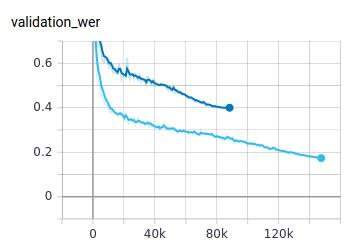
\includegraphics[width=100mm, keepaspectratio]{figures/architecture_comparrison.png}
\caption{LibriSpeech eredmények QuartzNet 5x1 (sötétkék) és 12x1 (világoskék) architektúrákon.}
\label{fig:TeXstudio}
\end{figure}

\section{Orosz nyelvű hálók}

Az orosz nyelvű implementációhoz már jó kiindulópontot jelentett a LibriSpeech-nél is alkalmazott architektúra. Az Mozilla Common Voice orosz adatbázisa átesett a szükséges formázásokon, és legeneráltam belőle a megfelelő .json fájlt. A legenerált fájlban odafigyeltem, hogy csak cirill betűk szerepeljenek, illetve szükség esetén kisbetűsítettem a szöveget.

\subsection{NeMo config fájl}

A NeMo a modellek leírásához config fájlokat használ. A fájlokban minden modellt és tanítást leíró paramétert meg lehet adni. Ezek közé tartozik a modell architektúrája, a használandó aktivációs rétegek, a learning rate és az epoch szám vagy az optimalizáló típusa.

Előnye, hogy könnyen módosítható és a programkódtól független. Megadhatók üresen hagyott paraméterek is, melyeket `???` el lehet jelölni. Ezeket később programkódból ki lehet tölteni, mint például a használandó manifest fájl elérési útját.

\subsection{Szükséges módosítások}

A config fájlban két dolgot kellett átállítani az orosz nyelv használata előtt. Az egyik maguk a betűk, label-ek voltak, mivel az orosz ábécé merőben eltér az angolétól. A cirill karakterek könnyen kinyerhető a google translate orosz nyelvű virtuális billentyűzete segítségével.

A másik átállítandó paraméter a config fájl AudioToTextDataLayer részében a leiratok normalizálására szolgáló rész\footnote{\url{https://github.com/NVIDIA/NeMo/issues/234}}. Erre azért van szükség, mert alapból elvégezné a modell, de szeretnénk elkerülni, mivel angol nyelvre lett tervezve így egyéb nyelveken nem működne megfelelően.

\subsection{Architektúrák}

A kísérletezéshez 2 különböző architektúrát, 12x1 és 15x5-et használtam. A választáson fő szempontja az volt, hogy ilyen architektúrákhoz rendelkeztem előre tanított angol nyelvű modellekkel. Ezeket később a transfer learning-nél használtam fel, és összehasonlítottam a véletlenszerűen inicializált súlyú modellek eredményeivel.

A tanításokat a Mozilla és Radio2 adatbázisán is futtattam. A Radio2-es adatbázis túl nagynak bizonyult, a hanganyagok méretét 8.7 másodpercben maximalizáltam, szemben a megszokott 16.7 másodperccel, így az összes tanítóadat 100 órát tett ki.

% 100 ÓRA HELYETT PONTOS ÉRTÉK!!!

Fontos kiemelni, hogy a tanítás közbeni pontosság teszteléséhez, azaz a validációhoz mindegyik esetben a Mozilla adatbázishoz tartozó tesztadatokat használtam. A pontosságot külön-külön megvizsgáltam a Radio2-es adatbázisból leválasztott, tanításhoz fel nem használt hanganyagokon is.

\subsection{Transfer learning}

A Transfer learning-hez előre betanított modelleket kellett szerezzek. A QuartzNet 15x5 architektúrájú modell könnyen elérhető volt, az Nvidia által szabad rendelkezésre volt bocsájtva. A 12x1-es architektúrát konzulensem Dr. Mihajlik Péter bocsájtott rendelkezésemre. Ez a modell kevesebb adaton és rövidebb ideig tanult mint a 15x5-ös, de jobb kiindulópont volt, aminek előállítására lehetőségem lett volna.

A modell betöltése hasonlóan történt a checkpoint-ból való folytatás betöltéséhez, azzal a különbséggel, hogy nem a teljese modellt használtam, csupán az encoder részét. Ez fontos különbség, hiszen a decoder használhatatlan lett volna, mivel az angol nyelvre lett tanítva. Így a decoder-hez véletlenszerűen inicializált súlyokat használtam, és a modell encoder részének súlyai kerültek átemelésre.

A tanítás ezen felül a megszokott szerint zajlott a megfelelő config fájl betöltésével, tanítóadatok és trainer beállításával, a súlyok kimentésével.